\subsection{Question 2: Rheology}

The different DS values for the differennt batches are calculated as

\begin{equation}
    DS = \frac{n_{\text{methacrylamide}}}{n_{\text{amine}}},
    \label{eq:DS}
\end{equation}

in which $n_{\text{amine}} = 0.385\unit{mmol}$ and

\begin{equation}
    n_{\text{methacrylamide}} = \frac{I(5.5\unit{ppm})+I(5.75\unit{ppm})}{2\cdot k},
    \label{eq:nMA}
\end{equation}

where $k$ is calculated as

\begin{equation}
    k = \frac{I(1\unit{ppm})}{6\cdot n_{\text{VLI}}},
    \label{eq:j}
\end{equation}

with $n_{\text{VLI}}=0.64\unit{mmol}$. All the data, from the NMR spectra on UFORA, and the calculated values are found in table \ref{tab:researcher1}.

\begin{table}[H]
    \centering
    \begin{tabular}{ccccccc}
      batch & $I(1\unit{ppm})$ & $I(5.5\unit{ppm})$ & $I(5.75\unit{ppm})$ & $k$ [1/mmol]& $n_{\text{methacrylamide}}$ [mmol] & DS [\%]\\
      \hline
      A & 142871.9 & 4918.98 & 4790.75 & 37206.22 & 0.130 & 34\\
      B & 166032.1 & 12362.5 & 12140.48 & 43237.53 & 0.283 & 74\\
      C & 114480.1 & 10858.83 & 1162.68 & 29812.83 & 0.369 & 96\\
    \end{tabular}
    \caption{DS values for the differennt batches}
    \label{tab:researcher1}
\end{table}

\begin{figure}[H]
    \centering
    \begin{subfigure}[b]{0.45\textwidth}
    \centering
    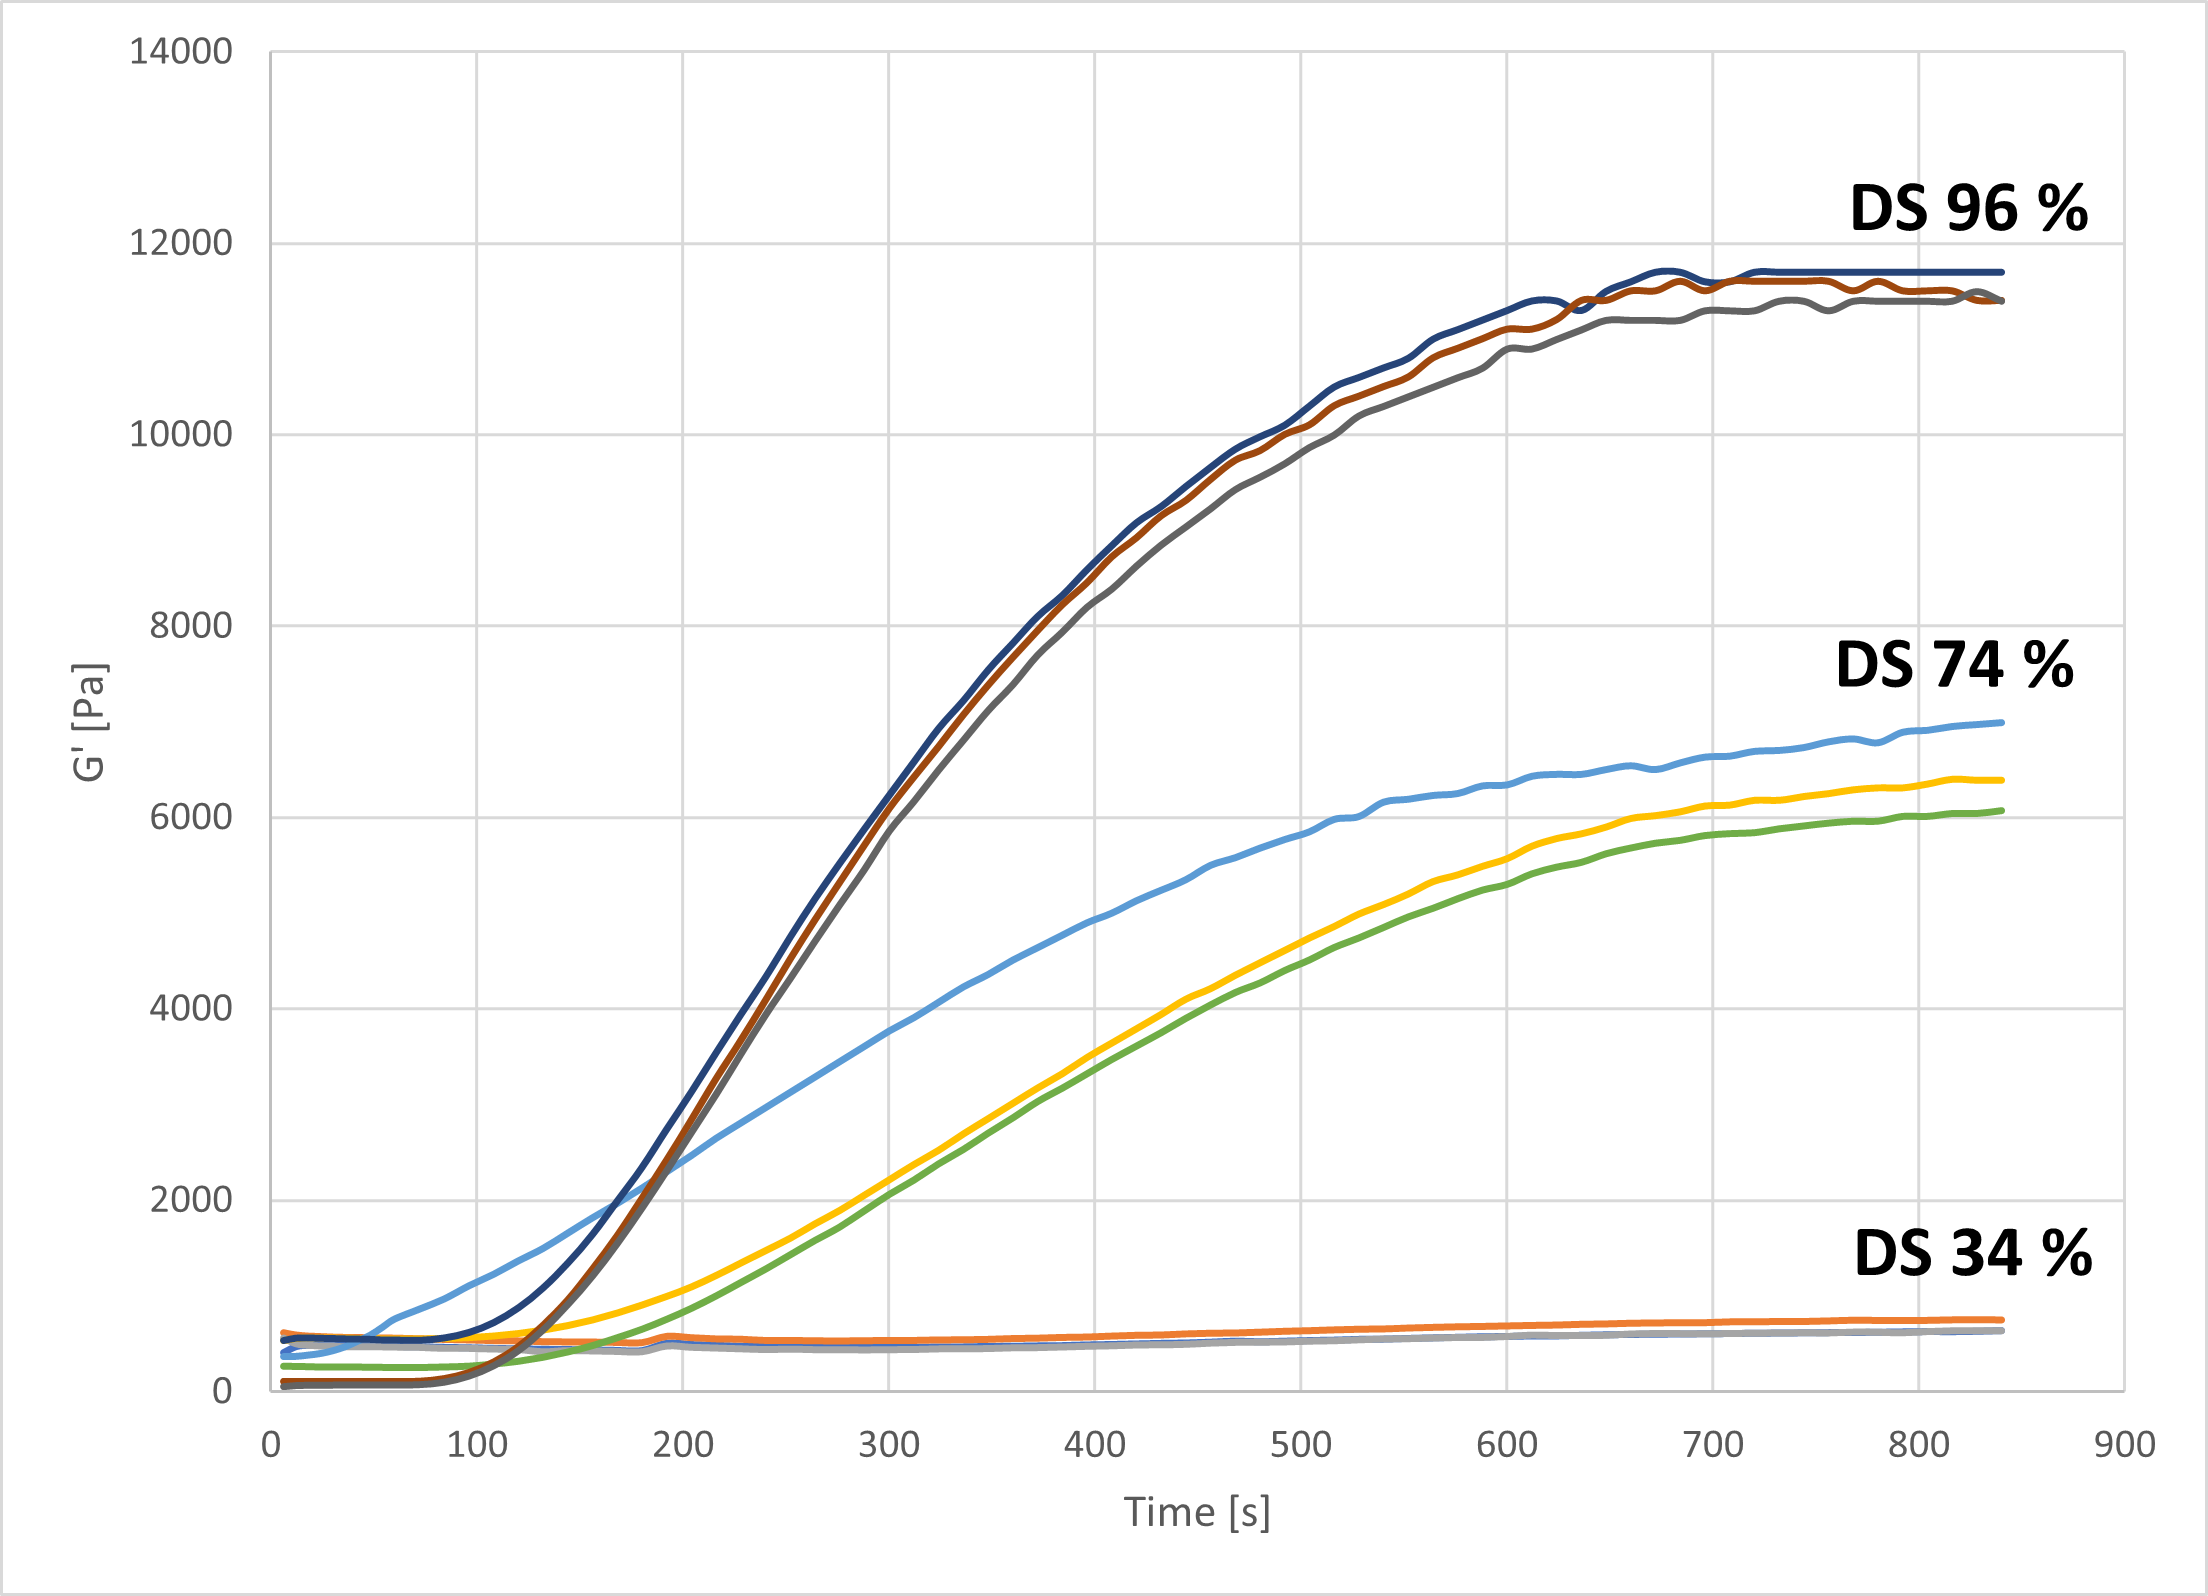
\includegraphics[width=\textwidth]{in_situ_UV_crosslinking_person1.png}
    \end{subfigure}
    \begin{subfigure}[b]{0.45\textwidth}
    \centering
    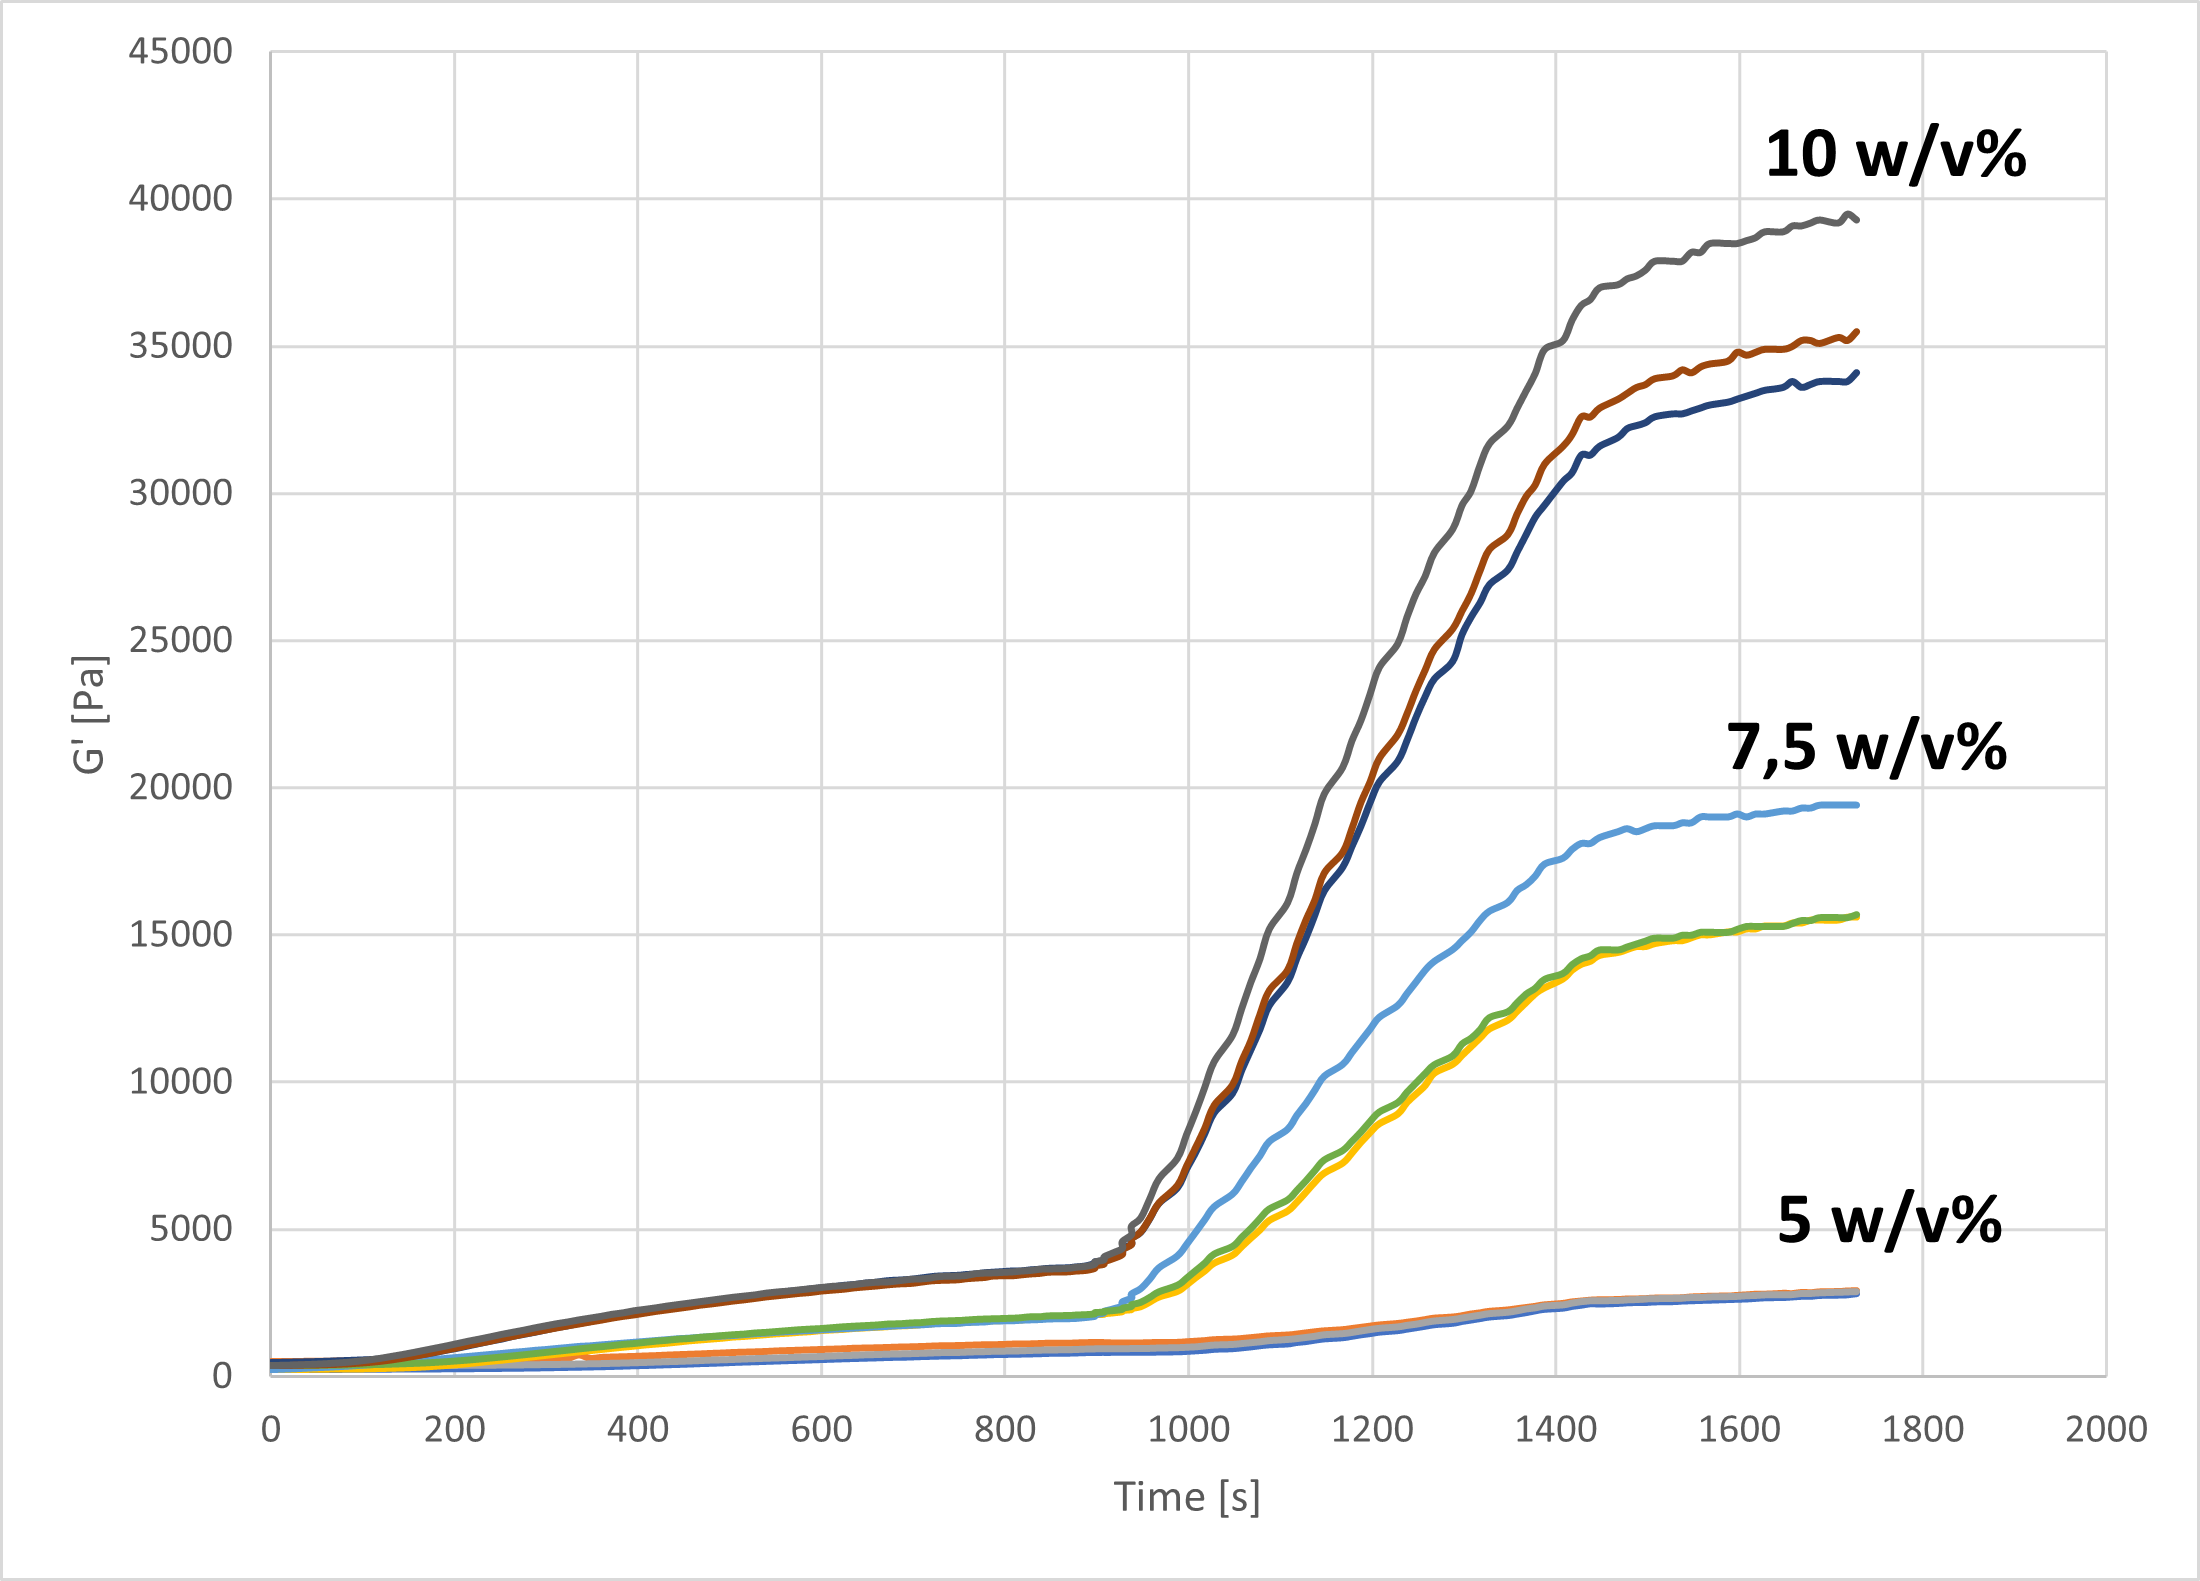
\includegraphics[width=\textwidth]{in_situ_UV_crosslinking_person2.png}
    \end{subfigure}
    \caption{Rheological in-situ UV-crosslinking with varying DS (right) and varying w/v\% (left)}
    \label{fig:rheo}
\end{figure}

Figure 2 displays rheological data from different researchers. The storage modulus $G'$ increases with increasing DS as well as with increasing w/v\%. $G'$ is a parameter that relates to the elasticity of the material obtained, indicating the amount of energy stored in the material due to deformation. Higher $G'$ values indicate that the material is stiff, while lower values indicate a more elastic behavior. In this rheology setup, gelMA is subjected to oscillating stress or strain while being irradiated by UV light, causing it to crosslink. $G'$ is measured during this crosslinking process, with more crosslinks implying a stronger force holding the material structure together. Higher DS values or higher concentrations of gelMA can induce more crosslinks. This theory corresponds perfectly with the obtained data. Furthermore, a steeper increase in $G'$ indicates a higher crosslinking speed. Once most of the gelMA is crosslinked, $G'$ reaches a plateau value.

A difference between the two measurements is apparent. The data from the left graph (researcher 1) was collected over a smaller time interval, and the maximum $G'$ is much lower compared to that of researcher 2, as both used batch C at 10 w/v\%. One possibility for this difference in measurement could be the amount of photo-initiator added to the gelMA. 

